\chapter{Framework} \label{ch:framework}
\minitoc% Creating an actual minitoc

\par In the previous chapter, we set the foundations of studying styles, which is the work done in the PhD. We explored our choices for generative models and the evaluation metrics, and how to ground them. We also had a discussion about lower- and upper-bound benchmarks. These foundations are necessary in order to have baselines to compare to, and performance aspects (i.e., metrics) use for this comparison. %\OSM{write a note about the fairness of selecting the baselines, and the reasoning behind them.}

\par In this chapter, we build on these foundations, by proposing the use of conditional temporal auto-encoder framework in order to study and extract styles, in the context of sequences (i.e., a time aspect exists in the data). We take advantage from the fact that the content is well known in our dataset (i.e., the identity of the letters in \textit{IRONOFF}).

\begin{mdframed}[backgroundcolor=blue!20]
    \begin{center}
        Questions addressed in this chapter
    \end{center}

    \begin{itemize}
        \item What possible framework to study styles? and why?
        \item How does this framework performance compare to the benchmarks?
        \item What kind of styles we can extract from this framework? and how do we extract them?
    \end{itemize}
\end{mdframed}

\clearpage

\section{Background}
  \subsection{What is an auto-encoder?}\label{sec:autoencoder}
  % \begin{itemize}
  %     \item General intro about auto-encoders
  %     \item Applications of static auto-encoder in image Reconstruction
  %     \item Temporal auto-encoder
  %     \item different ways to bias temporal encoders
  % \end{itemize}

  \par Auto-encoders~\citep{hinton2006reducing} is identity-capturing framework, that allow the emergence of interesting behaviors. To expand on this, the objective of the auto-encoder is to capture/learn the distribution of the input data (identity-capturing). An auto-encoder consists mainly of three parts (see figure~\ref{fig:autoenc}):
  \begin{enumerate}
    \item Encoder: it takes the input data, and project it into a manifold (the bottleneck).
    \item Bottleneck code/learned representation: this is the representation learned by the encoder. In the basic form, this just the output of some linear/non-linear activations. However, a lot of the literature exists on how to organize and shape the bottleneck, in order to allow the emergence of interesting information about the data.
    \item Decoder: it takes the learned representation, and reconstruct the original input from it.
  \end{enumerate}

  \begin{figure}
    \centering
    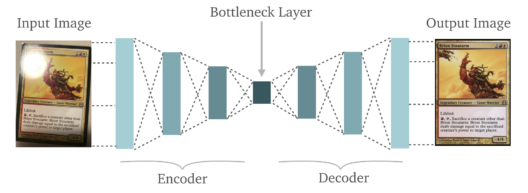
\includegraphics[scale=0.4]{images/framework/autoencoder.png}
    \caption{An example for the main components of an auto-encoder, used on image compression: an encoder takes the image, transfer it via a set of transformations into a bottleneck code, which is a compressed representation for that image. The decoder then takes this bottleneck code, and apply a series of transformations on it, in order to reconstruct the original input image. Source of this image is~\citep{autoencsimage}.}
    \label{fig:autoenc}
  \end{figure}


  \par There are many reasons for using auto-encoders, to name a few:
  \begin{description}
    \item [Dimensionality Reduction] It is one of the main motivations to study auto-encoders. By mapping a high-dimensional data into a smaller low-dimension space, we can better explore the data, or use it as a step in a pipeline of machine learning/data analysis operations, where it provides a more manageable format of the original data, as in~\citep{ha2018world}. It can also be used in classification system~\citep{Goodfellow-et-al-2016}.

    \item [Information Retrieval] The kind of search used in information retrieval is an efficient in low-dimensional space. In~\citep{salakhutdinov2009semantic}, auto-encoder is trained to produce low-dimensional binary code, which can be then used in queries (by returning the entities that have the same binary code).

    \item [Anomaly Detection] Multiple works have explored the use of auto-encoders in order to perform anomaly detection~\citep{sakurada2014anomaly,an2015variational,ribeiro2018study}. The main hypothesis is that the auto-encoder will learn the most salient features in the data. Thus, when faced with an anomaly, a significant degradation in the quality of reconstruction will be noticed. The reconstruction error can be used in this case as an indicator if the input data point is an anomaly or not.

    \item [Image De-noising] Multiple works have explored the use of auto-encoder in order to de-noise images~\citep{cho2013boltzmann,cho2013simple,gondara2016medical}. The applications of image de-noising are diverse, from post-processing of digital images, to more sensitive areas like medical images.

    % \item [Exploring the data via bottleneck behavior]: with a compact representation of the high-dimensional input, it is interesting to explore the different characteristics of the data with traditional tools, like visualization and clustering.
  \end{description}

  \par The idea of compressing data is not new. Techniques like \textit{Principal Components Analysis} (PCA)~\citep{jolliffe2011principal} or \textit{Independent component analysis} (ICA)~\citep{hyvarinen2000independent} do exist in order to project the data into smaller dimensions. But they are usually restricted by several assumptions. In case of PCA, it assumes linearity and orthogonality in the dimensions of variation in the data. Neural networks enables us to get around this issue, by leveraging nonlinearity and multiple layers, this giving us a more flexible approach to find dimensions of variation in the data.

  \subsection{Sequence auto-encoder}
    It a special case of auto-encoder, where RNN is used in order to compress a sequence into a fixed size bottleneck code. The sequence itself could have a varied size. The first architecture proposed for sequence auto-encoder was proposed in~\citep{cho2014learning,sutskever2014sequence}, with statistical machine translation as the main application. They use RNN encoder and decoder parts, and consider that the last hidden state of the RNN encoder to be the summary/compression of the sequence. The RNN decoder uses this bottleneck in order to reconstruct the whole original sequence (see figure~\ref{fig:seq2seq}).

    \begin{figure}
      \centering
      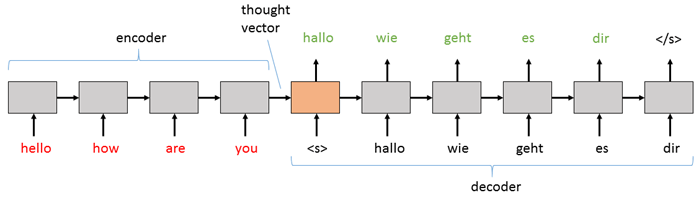
\includegraphics[scale=0.8]{images/framework/SequencetoS2.png}
      \caption{An illustration for a sequence-to-sequence architecture, used for language translation between English and German. The encoder summarize the English sentence, and the decoder use it as to bias its own output, to generate the equivalent German sentence.}
      \label{fig:seq2seq}
    \end{figure}

    \par There many applications where a sequence-to-sequence model is used, for example:
    \begin{description}
      \item [Machine translation]~\citep{sutskever2014sequence} used sequence-to-sequence architecture in order to develop a machine translation system that surpassed the published results to that moment. The first sequence is the source language, and the second sequence is the target language (that can also differ in the word count from the source language).
      \item [Speech synthesis] Speech synthesis also benefited from a sequence-to-sequence architecture, like the work done in~\citep{oord2016wavenet,wang2017tacotron}, achieving currently the state-of-the-art results. Another common approach for sequence-to-sequence learning is to use convolution network instead of RNN for the encoder and/or the decoder, like the work done in~\citep{ping2017deep}. A convolution network is generally faster than RNN and parallelize better, thus making it a lucrative approach. The underlying assumptions are the same however.
      \item [Video captioning] Another application that benefited from sequence-to-sequence architecture is generating text (sequence of words/letters) that describe a video (sequence of frames), as nicely summarized in~\citep{aafaq2018video}. In this case, the encoder -- dealing with the video part -- is usual a convolution neural network (because of its excellent ability to capture spatial features), while the encoder -- dealing with the text part -- is usually a RNN.
    \end{description}

  \subsection{Conditioned auto-encoder}
    \par In the examples mentioned before, we focused on unconditional auto-encoder, where in the decoder only have the information given to it from the encoder part. A conditioned auto-encoder is when we concatenate extra information to the output of the encoder, and feed it to the decoder\footnote{The word 'conditioned' is used when a neural network has information from about the task. So a decoder is a conditioned network on the encoder information. We distinguish here in the terminology between 'unconditioned auto-encoder', where the decoder is not conditioned on anything else except the encoder, and 'conditioned auto-encoder' where the decoder has access to extra information other than the encoder.}. Why conditioning an auto-encoder? It frees the encoder from learning the condition information -- since this information is given for free -- , allowing it to focus on other parts.

    \par An example of this is the work done in~\citep{van2017neural}, where they used an auto-encoder to compress audio, and condition the decoder on the speaker-id. This led the encoder to factor out speaker-specific information in the learned bottleneck, thus, learning speaker-independent information\footnote{Simple explanation and demonstration for that paper can be found in \url{https://avdnoord.github.io/homepage/vqvae/}}.

\section{Putting it all together}
  \par In order to address the research questions stated at the beginning of the chapter, we chose to adopt the concept of conditioned auto-encoder as our framework to explore styles in handwriting, for the potential following benefits discussed in the previous section:
  \begin{itemize}
    \item Conditioning the decoder on the content identity of the task (i.e., the letter identity) will free the encoder from learning this information, thus allowing it to focus on learning the letter-independent style relevant information.
    \item The encoder will learn a bottleneck, that is a compressed information about the sequence style. This can allow us to explore this bottleneck via traditional techniques (PCA, tSNE, clustering, classification of the bottleneck...etc), thus, getting more insight about what the model actually learned
  \end{itemize}

  \par In this following subsections, I will present our contributions: the model architecture we used, and quantifying the quality of the generated letter using the evaluation metrics and benchmarks we discussed in the previous chapter. Then, we will briefly take a look at our first attempt to tackle transfer learning\footnote{More details on transfer learning in the next chapter}. I then end with the style extraction part, where we explore what knowledge/information about the styles our model has extracted. The work done in this chapter was published in~\citep{icaart19}.

  \subsection{Model architecture}
     \par The model architecture is illustrated in figure~\ref{fig:model_arch}. The input/output frames of the model are detailed in figure~\ref{fig:input_shape}. The tracing of the letter is first fed to the encoder module. The final hidden state of that module summarizes the letter. In order to allow this module to focus on learning the style embedding, we complement this last hidden state with the one-hot encoding of the letter identity, and use an embedding of them as the bias input to the generator. The encoder thus is free from the need to learn the letter identity, and can focus learning the style information that enables the generator to better approximate the ground truth tracings.

    \par In the decoder, we follow the framework proposed by \cite{vinyals2015show} in order to bias the model -- as in the previous chapter -- : we create an extra time step at the beginning, which has the information we want to bias the model with. In this case, this time step (34-D) is the projection of the encoder last hidden state (128-D) and the letter encode (26-D). This has a much lower dimension than encoder hidden state. This further encourage the model to learn only the necessary style information, as suggested in \cite{DBLP:journals/corr/abs-1803-09047}.

    \begin{figure}[htbp!]
      \centering
      \begin{subfigure}{1.0\textwidth}
        \centering
        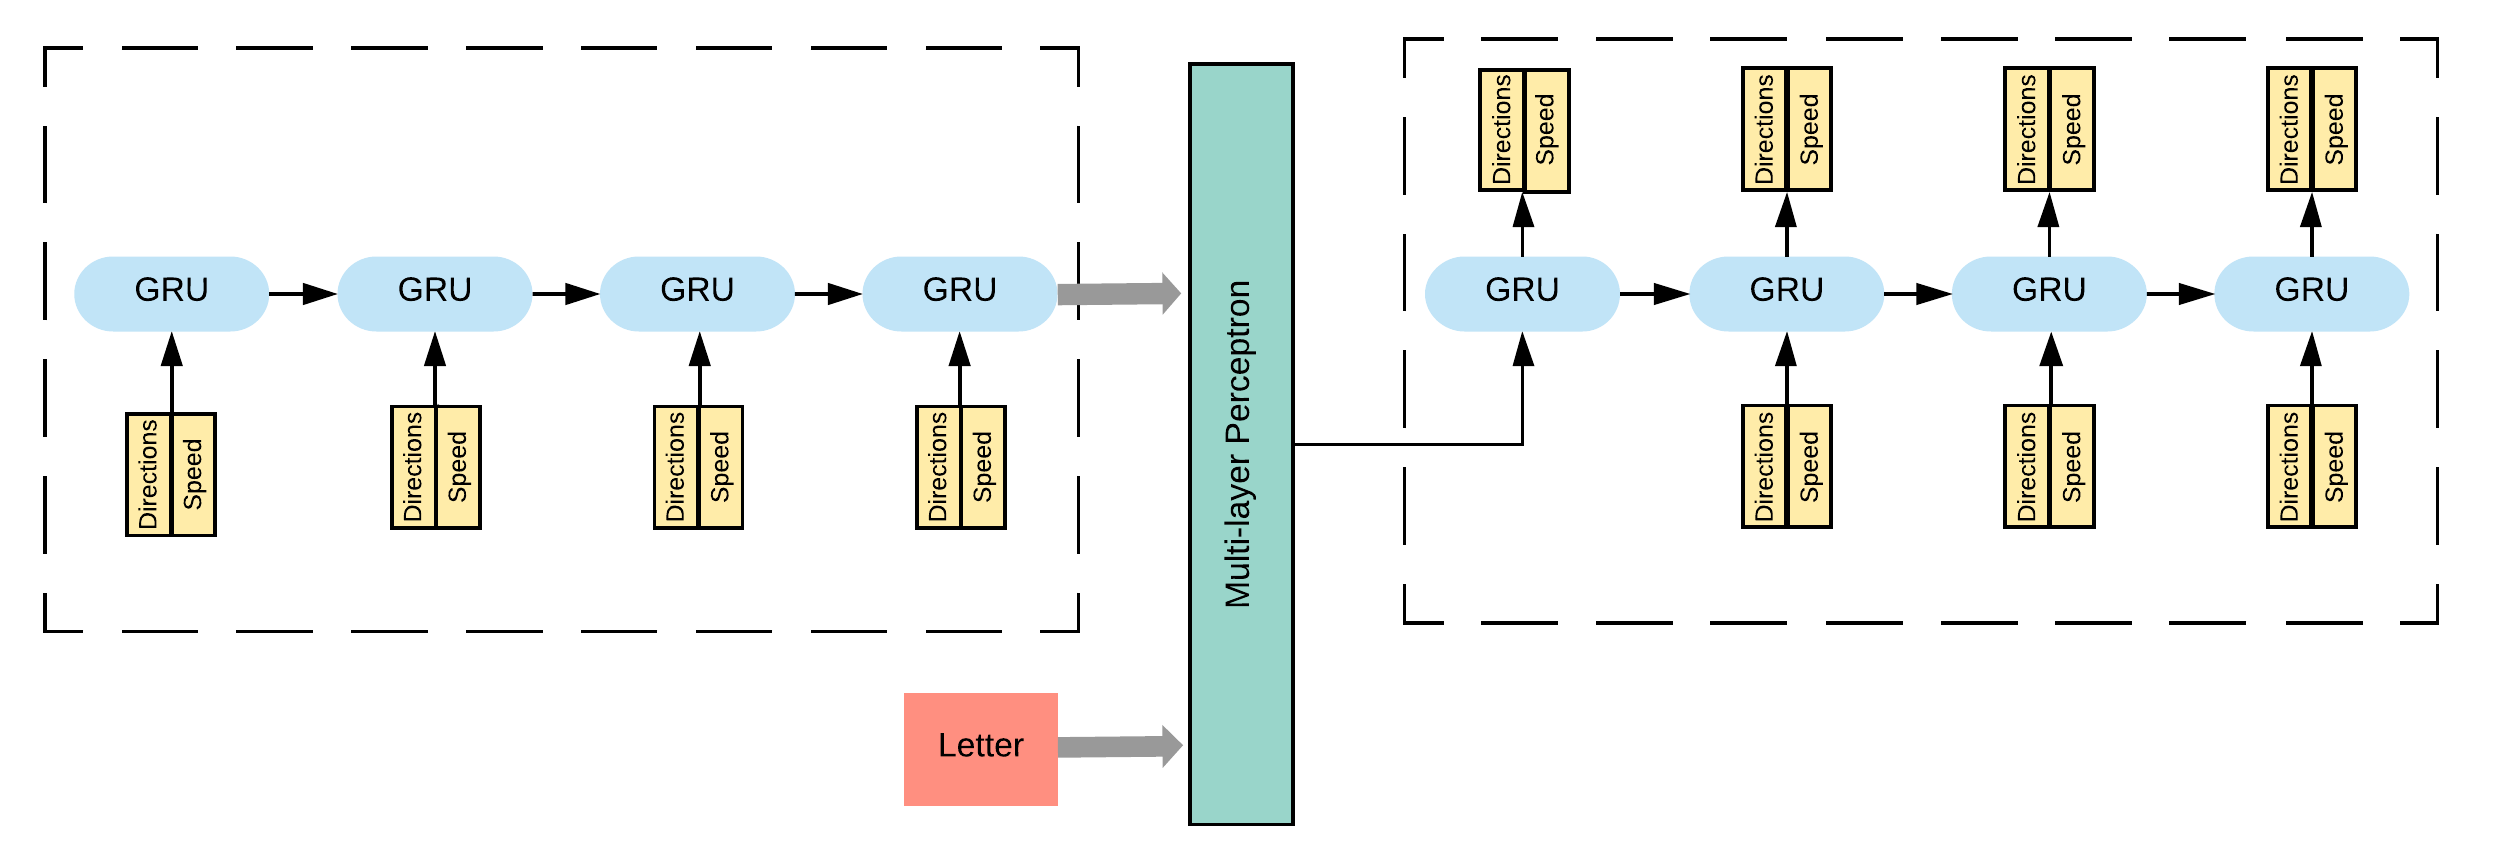
\includegraphics[scale=0.7]{images/framework/training_mode.png}
        \caption{Training mode\label{fig:training_mode}, using the \textit{teacher forcing} methodology~\citep{Williams:1989:LAC:1351124.1351135,Goodfellow-et-al-2016}.}
      \end{subfigure}
      % \vfill
      \begin{subfigure}{1.0\textwidth}
        \centering
        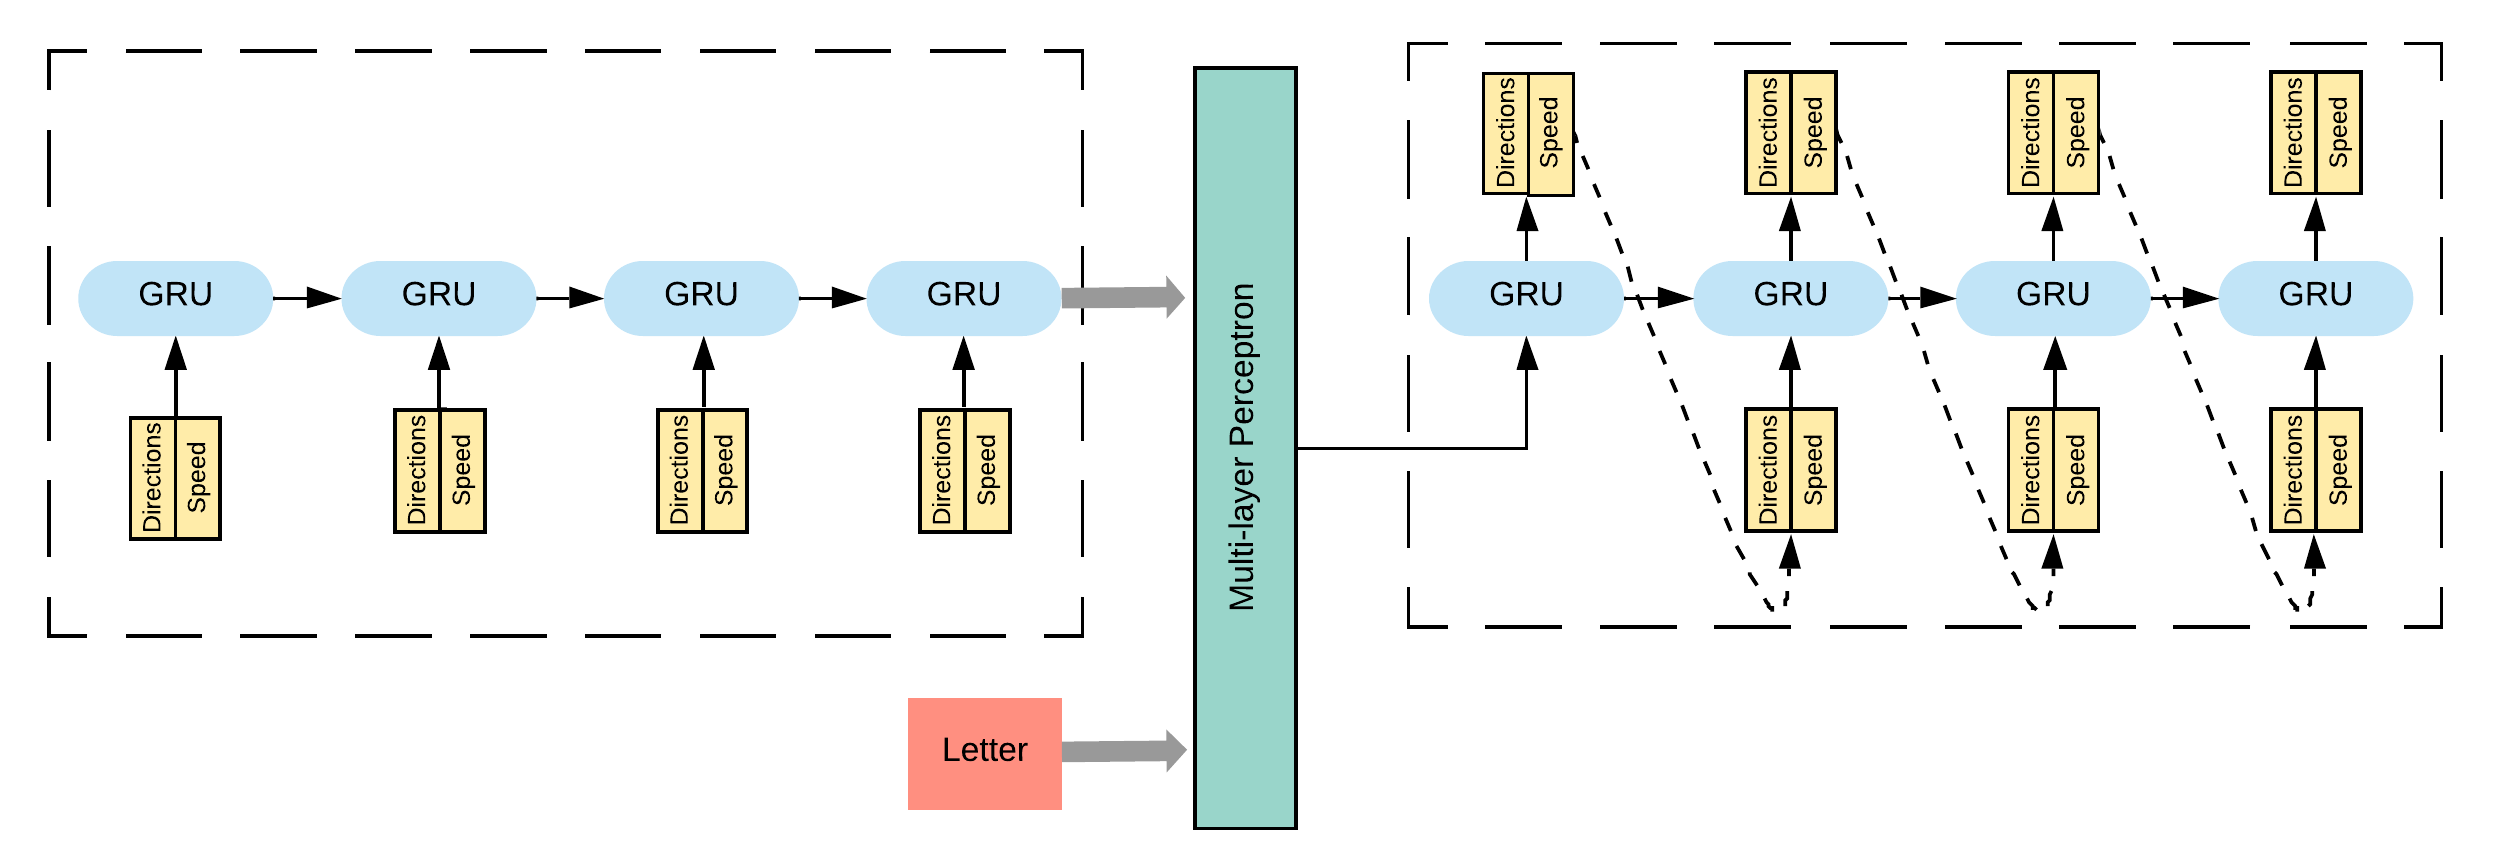
\includegraphics[scale=0.7]{images/framework/inference_mode.png}
        \caption{Inference mode\label{fig:inf_mode}, using the \textit{softmax temperature sampling} method.}
      \end{subfigure}
      \caption{Schematic diagram of the model we used. During the training time~\ref{fig:training_mode}, the input to the model is always the ground truth. During the inference time~\ref{fig:inf_mode} however, the input to the decoder (generator) part at each time step is its own predication in the previous time step.}
      \label{fig:model_arch}
    \end{figure}

    \begin{figure}[htbp!]
      \centering
      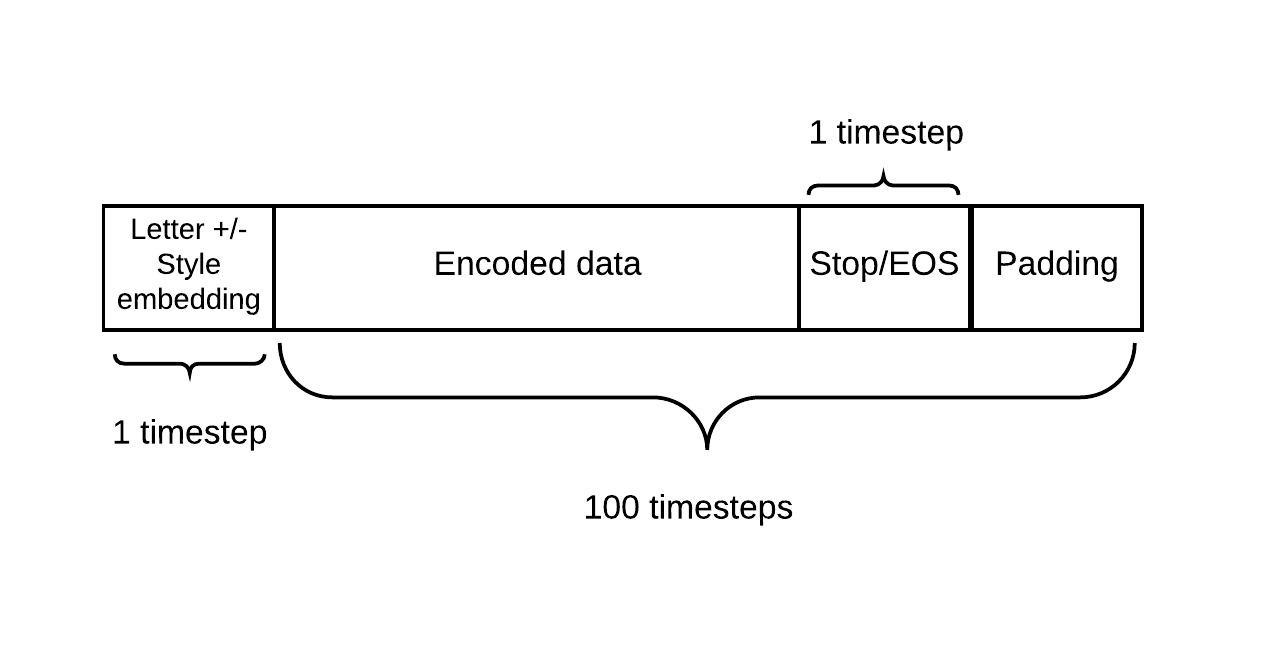
\includegraphics[scale=1.0]{images/framework/input_shape.jpeg}
      \caption{Input sequence to our model. The first time step contains the information necessary to condition/bias our model. In case of the encoder, this first time step (the bias) is not included.}
      \label{fig:input_shape}
    \end{figure}


    \par In order to allow for faster exploration of different hyper-parameters, we use an early stopping of 20 epochs (when no improvement in the validation score happens during these epochs). To summarize, the current model specifications:
    \begin{itemize}
        \item Encoder hidden size: 128
        \item Decoder hidden size: 128
        \item Encoder layers: 2
        \item Decoder layers: 2
        \item Encoder dropout: 0.0
        \item Decoder dropout: 0.2
        \item Learning rate: 0.001
    \end{itemize}

  \subsection{Letter generation with style preservation}
  \par The objective here to compare the quality of the generated letters to the state-of-the-art benchmarks. As mentioned earlier, we compare using the BLEU score metric and the EoS analysis.
  The BLEU score results can be seen in table~\ref{table:bleu_gen}, and the results for EoS analysis results are in table~\ref{table:EoS_gen}. We can see that the BLEU-3 score results of our model achieves 32.3\% accuracy in Speed feature and 38.7\% accuracy in Freeman feature, compared to 25.1\% and 28.3\% accuracy using the benchmark model on both features respectively.
  \par The same goes for the EoS analysis. In comparing the Person Coefficient, our model achieves 0.99 score compared to 0.55 for the benchmark model (the highest score is 1.0). This is a support that our model capture the style of handwriting better than the benchmark.
  \par Examples for generated letters can be found in figure~\ref{fig:letters_examples}.


  \begin{table}[!htbp]
  \centering
  \begin{tabular}{l|c c c|c c c}
  \hline
  \multicolumn{1}{c|}{Aspect/Feature} & \multicolumn{3}{c|}{ Speed } & \multicolumn{3}{c}{ Freeman }   \\ \hline
  Model / B-score      & B-1  & B-2  & B-3           & B-1  & B-2   & B-3              \\ \hline
  Letter + Writer bias & 51.5 & 41.4 & 25.1          & 56.7 & 39.4  & 28.3             \\\hline
  \textbf{Style Extractor} & \textbf{71} & \textbf{51.7} & \textbf{32.3} & \textbf{65.6} & \textbf{51.5} & \textbf{38.7} \\\hline
  \end{tabular}
  \caption{BLEU scores for different models for known writers.}
  \label{table:bleu_gen}
  \end{table}

  \begin{table}[!htbp]
  \centering
  \begin{tabular}{l|c c c|c c c}
  \hline
  \multicolumn{1}{c|}{Aspect/Feature} & \multicolumn{3}{c|}{ Speed } & \multicolumn{3}{c}{ Freeman }   \\ \hline
  Model / B-score      & B-1  & B-2  & B-3           & B-1  & B-2   & B-3              \\ \hline
  Letter + Writer bias & 55.4 & 39.6 & 25.3 & 50.2 & 38.6 & 27.7             \\\hline
  \textbf{Style Extractor} & \textbf{72.4} & \textbf{52.4} & \textbf{32.2} & \textbf{70.4} & \textbf{55.6} & \textbf{42.1} \\\hline

  \end{tabular}
  \caption{BLEU scores for different models for style extraction for 30 new writers (style transfer).}
  \label{table:bleu_transfer}
  \end{table}

  % \begin{table}[!htbp]
  % \centering
  % \begin{tabular}{|l|c|c|}
  % \hline
  % Models & Pearson coefficient & p value \\ \hline
  % Letter + Writer bias & 0.55 & 0.04\\ \hline
  % \textbf{Style Extractor} & 0.99 & 0.01 \\ \hline
  % \end{tabular}
  % \caption{Pearson correlation coefficients and associated p-values for the End-Of-Sequence (EoS) distributions for the different models: a) The results in a normal generation scenario. b) The results on 30 new writers (style transfer).}
  % \label{table:EoS_gen}
  % \end{table}

  \begin{table}[!htbp]
  \centering
  \begin{tabular}{l|c}
  \hline
  Models & Pearson coefficient\\ \hline
  Letter + Writer bias & 0.55\\ \hline
  \textbf{Style Extractor} & \textbf{0.99} \\ \hline
  \end{tabular}
  \caption{Pearson correlation coefficients for the End-of-Sequence (EoS) distributions for the conditioned-autoencoder framework (style extractor) compared to the baseline (with letter and writer information only), on the generated letters compared to the ground truth. We can see that the (style extractor) outperforms the baseline.}
  \label{table:EoS_gen}
  \end{table}

  % \begin{table}[!htbp]
  % \centering
  % \begin{tabular}{|l|c|c|}
  % \hline
  % Models & Pearson coefficient & p value \\ \hline
  % Letter + Writer bias & 0.5 & 0.7 \\ \hline
  % \textbf{Style Extractor} & 0.99 & 1.4e-29\\ \hline
  % \end{tabular}
  % \caption{Pearson correlation coefficients and associated p-values for the End-Of-Sequence (EoS) distributions for the different models: a) The results in a normal generation scenario. b) The results on 30 new writers (style transfer).}
  % \label{table:EoS_transfer}
  % \end{table}

  \begin{table}[!htbp]
  \centering
  \begin{tabular}{l|c}
  \hline
  Models & Pearson coefficient\\ \hline
  Letter + Writer bias & 0.5\\ \hline
  \textbf{Style Extractor} & \textbf{0.99}\\ \hline
  \end{tabular}
  \caption{Pearson correlation coefficients for the End-Of-Sequence (EoS) distributions for the different models on 30 new writers (style transfer). Even though the baseline model is given explicit information about the writer, the style extractor still outperforms the baseline. This could be an indication that the there is a limited number of styles after-all.}
  \label{table:EoS_transfer}
  \end{table}

  \subsection{Style transfer}
  \par One of the hypotheses we want to test is whether there is a limited number of styles needed, to generalize over new writers. To achieve this, the learned representation for styles should extract generic information about the styles.

  \par In order to test this hypothesis, we expose our model to 30 writers that have not been seen before. We compare our model performance on these writers with a model biased by the writer and letter identities (the benchmark model). The latter model was not constrained from seeing those writers (thus, the reported results of the comparison overestimates the actual performance of that model).

  \par The BLEU scores can be seen in table~\ref{table:bleu_transfer}. Our model achieves on BLEU-3 score 32.2\% and 42.1\% accuracy on the Speed and Freeman code features, compared to 25.3\% and 27.7\% on the benchmark model for the same features respectively.
  \par The EoS analysis can be seen in table~\ref{table:EoS_transfer}. Our model achieves a Pearson coefficient value of 0.99, compared to 0.5 for the benchmark.
  Thus, the new model clearly outperform the current benchmarks on the transfer task, on both BLEU score and EoS analysis.

  \subsection{Styles per letter} \label{ch:framework_sec:styleperletter}
  \par One of the nice consequences of using our model is that we can have a better look at the styles. We explore the latent space for multiple letters, and see that we can uncover interesting writing styles. A full scale analysis is beyond the scope of this thesis. We project the latent space using \textit{Principal Components Analysis} (PCA)~\citep{jolliffe2011principal} and t-SNE~\citep{maaten2008visualizing}.

  \par As a start, we take a look at letter X. Beforehand, we identified a style feature in letter X: some writer draw X clockwise, and some draw it anti-clockwise\footnote{We did not find a connection between this point and the handiness of the participants.}. We manually annotated the whole dataset for this feature; the result can be seen in figure~\ref{fig:x_rotation}. Almost half of the writers draw the letter X clockwise, and the other half draw it anti-clockwise. If our assumption is correct, our model should be able to capture this feature. We project the latent  of the model using PCA on all the letter X, which can be seen in figure~\ref{fig:x_bottleneck}. The model latent space clusters almost perfectly match those based on rotation. Examples for letters from both clusters are in figure~\ref{fig:examples_x}.

  \par Encouraged by the results on letter X, we explored more letters. For letter C, we can see the latent space project in figure~\ref{fig:c_letter}. It can be seen that there are at least two main clusters. Examples from this cluster in the red ellipse are in figure~\ref{fig:examples_c}. This clearly represents the Edwardian handwriting style. The rest of the writers (in the big cluster) have a very similar style (this is expected, since the drawing of the letter C is quite simple).

  \par For letter A, our model latent space create two main clusters, figure~\ref{fig:a_bottleneck}. We give examples from those two in figure~\ref{fig:examples_a}, where we can see clear difference in the style. Some people start drawing the letter from down-left, other writers start from the top of letter A, move down, then continue drawing of the letter.

  \par Another example is for letter S bottleneck, figure~\ref{fig:s_bottleneck}. There are three resulting clusters which we investigated. The indicated cluster (in red) is clearly different from the other two clusters (not indicated). Examples can be seen in figure~\ref{fig:examples_s}. The indicated cluster is again for people with Edwardian handwriting style. We did not find a clear difference between the other two clusters though, but this is an expected outcome of using t-SNE (since it does not have the clear objective of clustering styles).

  \par These examples show is that we can use our model to extract verbose style information.
  \begin{figure}[htbp!]
      \centering
      \fbox{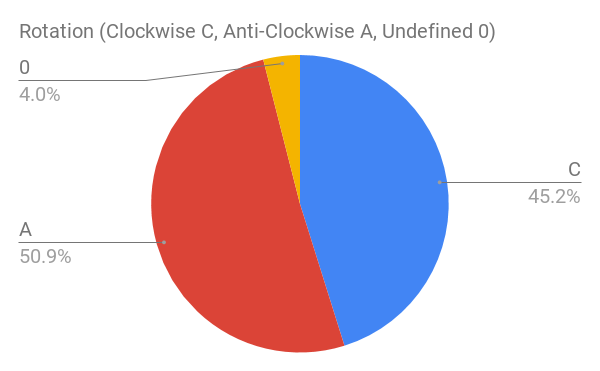
\includegraphics[scale=0.5]{images/framework/x_rotation.png}}
      \caption{Results of the manual annotation for the rotation of letter X drawings over the whole dataset. Almost half the writers drew X clockwise, the other half anti-clockwise. The undefined styles were unclear to determine.}
      \label{fig:x_rotation}
  \end{figure}

  \begin{figure}[htbp!]
      \centering
      \fbox{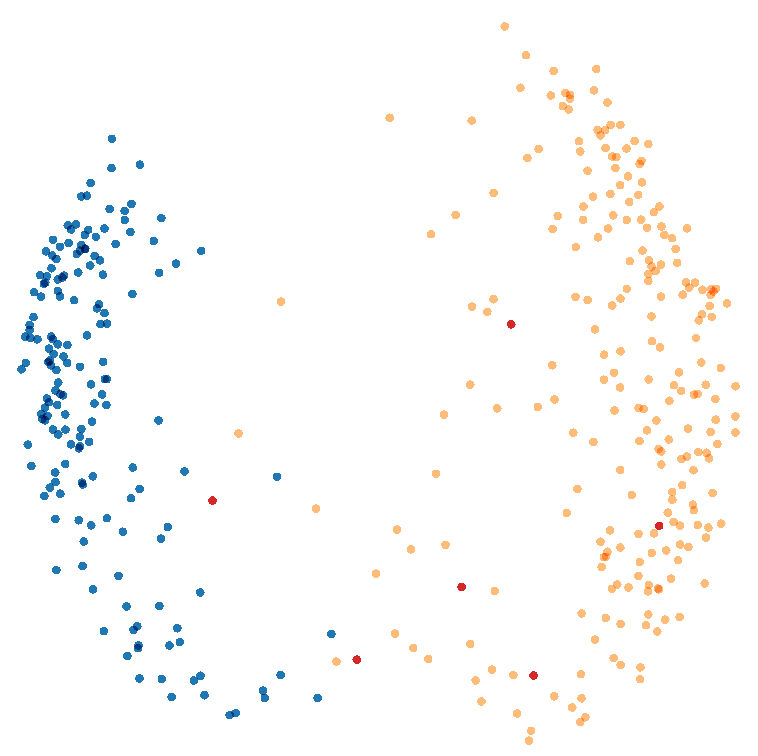
\includegraphics[scale=0.26]{images/framework/x_bottleneck.png}}
      \caption{Projection for latent space for letter X using PCA. The colors show the ground truth of the X rotation: blue is counter clockwise, orange is clockwise, and the few red points are undefined.}
      \label{fig:x_bottleneck}
  \end{figure}

  \begin{figure}[!htbp]
      \centering
      \begin{subfigure}{0.45\textwidth}
          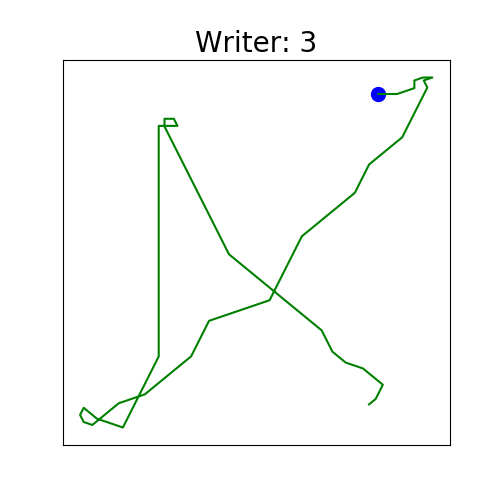
\includegraphics[scale=0.50]{images/framework/X_3.png}
      \end{subfigure}
      \hspace{0.5em}
      \begin{subfigure}{0.45\textwidth}
          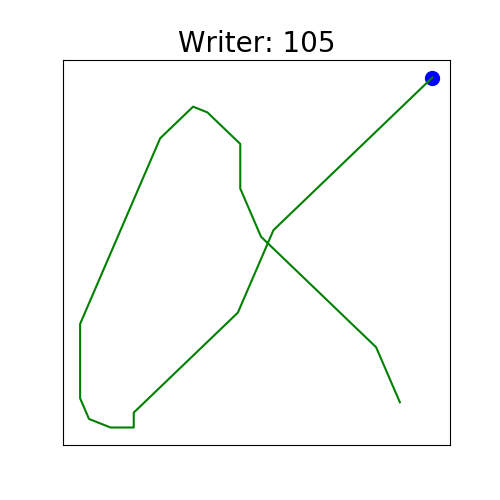
\includegraphics[scale=0.50]{images/framework/X_105.png}
      \end{subfigure}
      \vspace{1em}
      \begin{subfigure}{0.45\textwidth}
          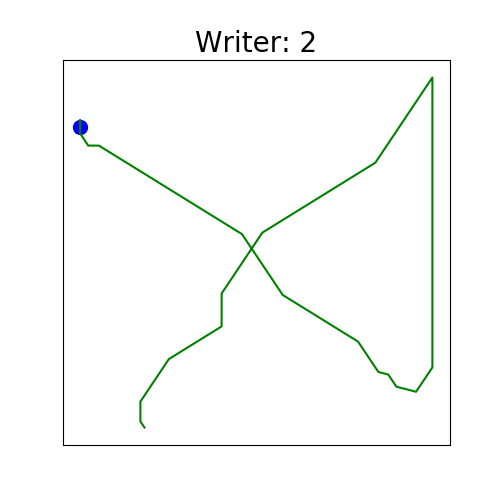
\includegraphics[scale=0.50]{images/framework/X_2.png}
      \end{subfigure}
      \hspace{0.5em}
      \begin{subfigure}{0.45\textwidth}
          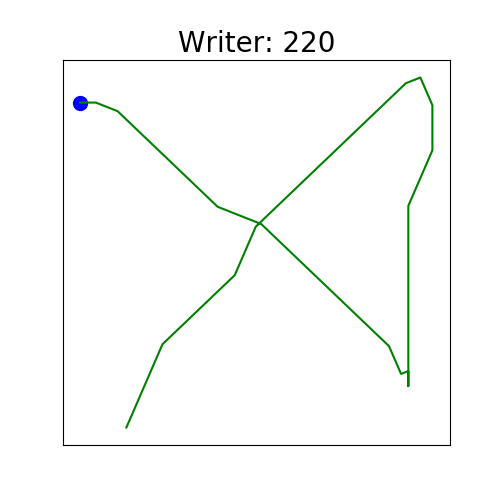
\includegraphics[scale=0.50]{images/framework/X_220.png}
      \end{subfigure}

      \caption{Examples for writing of letter X. Starting point is marked with the blue mark. Each raw is randomly sampled from each cluster in the bottleneck. The clusters shows that almost half the writers draw the letter clockwise (first row, first cluster), and the other half draw it anti-clockwise (second row, second cluster).}
      \label{fig:examples_x}
  \end{figure}

  \begin{figure}[htbp!]
      \centering
      \fbox{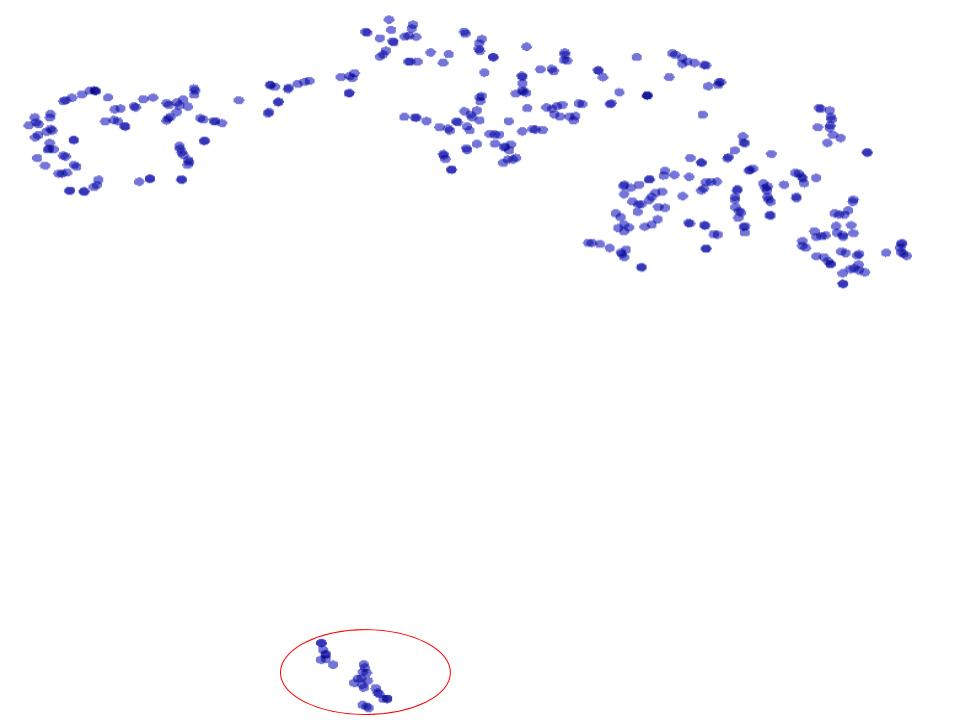
\includegraphics[scale=0.40]{images/framework/Cletter_2.jpg}}
      \caption{Projection for latent space for letter C using t-SNE. The cluster surrounded by the red circle has a clear interpretation, where writers have a cursive style.}
      \label{fig:c_letter}
  \end{figure}

  % \begin{figure}[htbp!]
  % \centering
  % \fbox{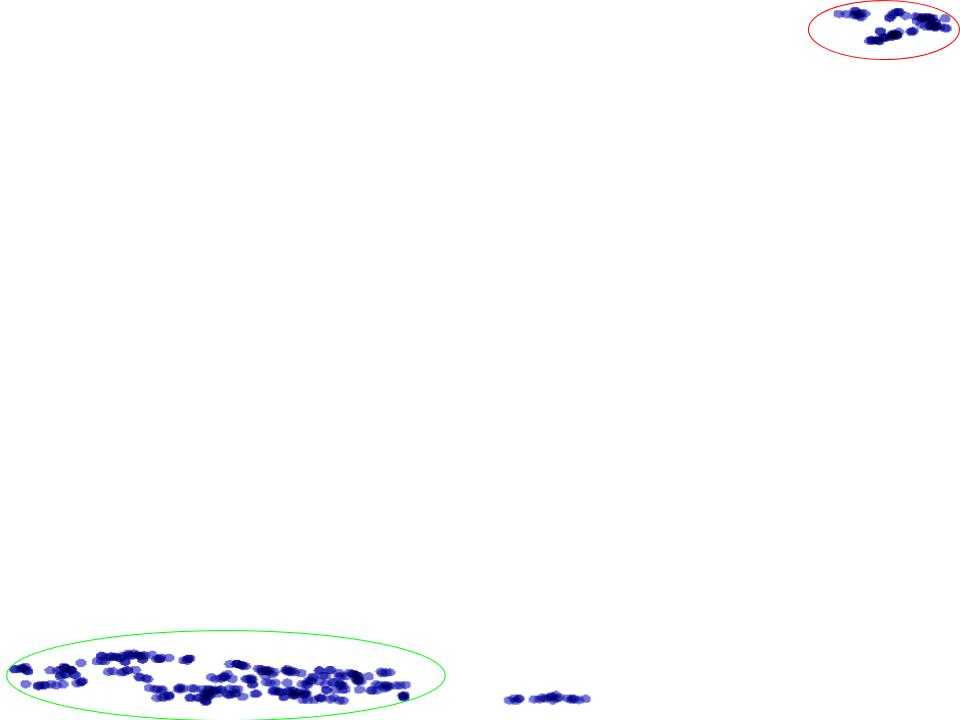
\includegraphics[scale=0.20]{a_bottleneck.jpg}}
  % \caption{Projection for bottlenecks for letter A using t-SNE.}
  % \label{fig:a_bottleneck}
  % \end{figure}

  \begin{figure}[htbp!]
      \centering
      \fbox{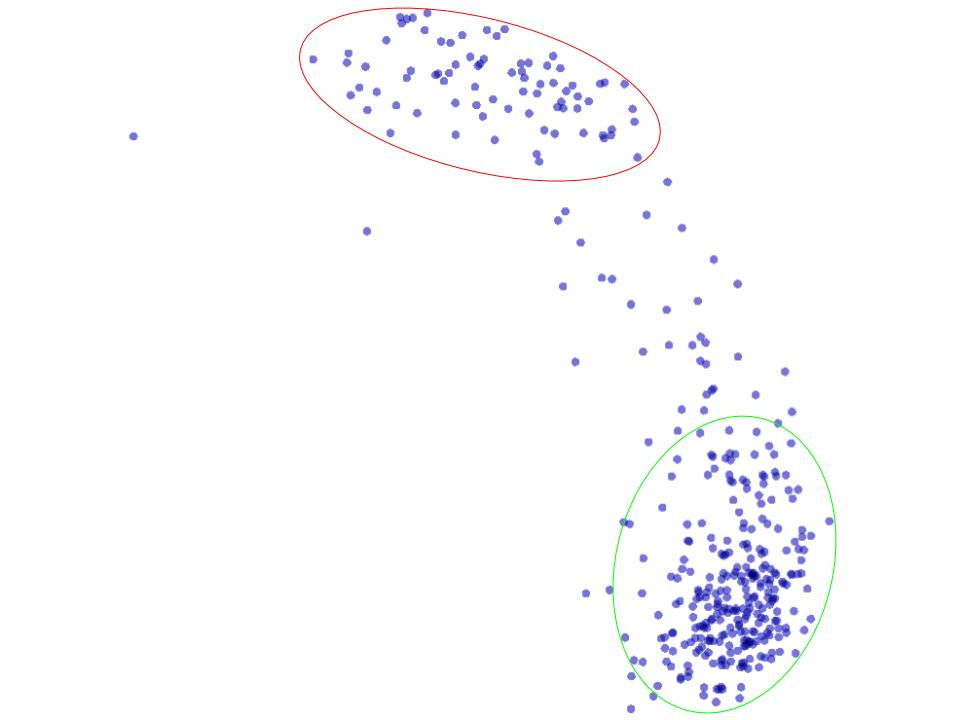
\includegraphics[scale=0.40]{images/framework/comparison_figures/letter_a_bottleneck.jpg}}
      \caption{Projection for latent space for letter A using PCA.}
      \label{fig:a_bottleneck}
  \end{figure}

  \begin{figure}[!htbp]
      \centering
      \begin{subfigure}{0.45\textwidth}
          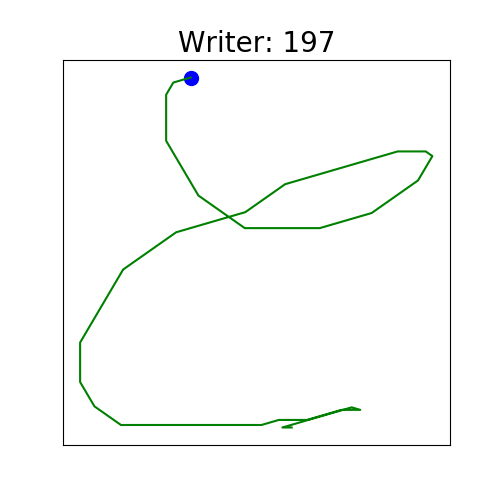
\includegraphics[scale=0.50]{images/framework/C_197.png}
      \end{subfigure}
      ~
      \begin{subfigure}{0.45\textwidth}
          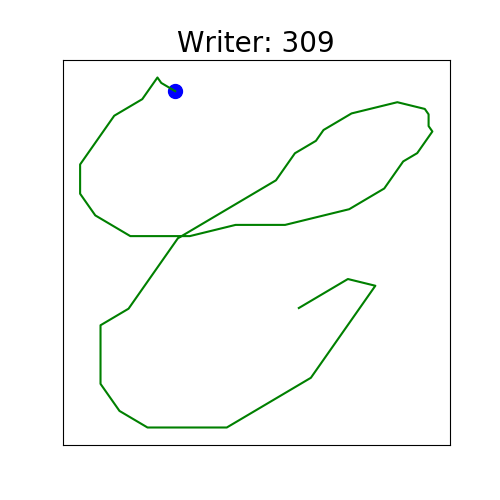
\includegraphics[scale=0.50]{images/framework/C_309.png}
      \end{subfigure}
      ~
      \begin{subfigure}{0.45\textwidth}
          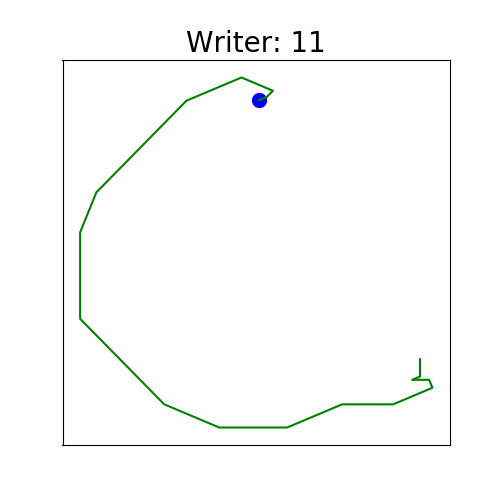
\includegraphics[scale=0.50]{images/framework/C_11.png}
      \end{subfigure}
      ~
      \begin{subfigure}{0.45\textwidth}
          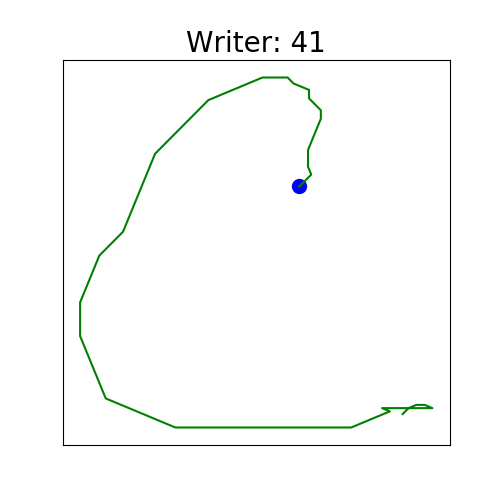
\includegraphics[scale=0.50]{images/framework/C_41.png}
      \end{subfigure}

      \caption{Examples for writing of letter C from the selected cluster (first row) versus the rest of the letter drawings (second row). Starting point is marked with the blue mark. The drawings from the selected cluster show people with Edwardian style of handwriting.}
      \label{fig:examples_c}
  \end{figure}

  \begin{figure}[!htbp]
      \centering
      \begin{subfigure}{0.45\textwidth}
          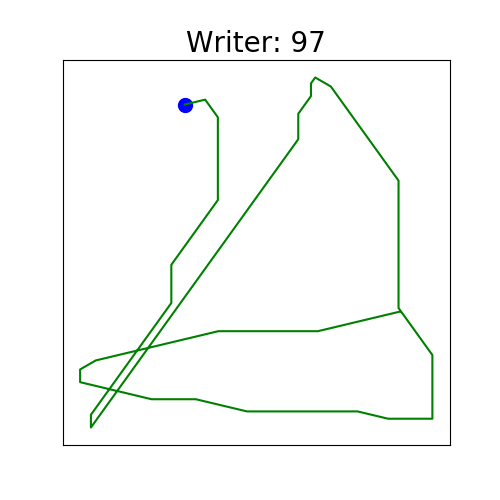
\includegraphics[scale=0.50]{images/framework/A_97.png}
      \end{subfigure}
      ~
      \begin{subfigure}{0.45\textwidth}
          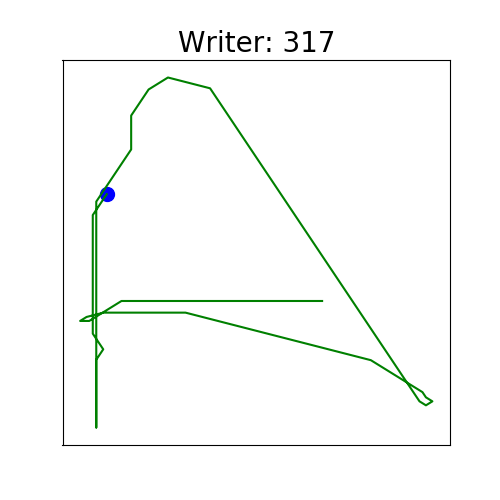
\includegraphics[scale=0.50]{images/framework/A_317.png}
      \end{subfigure}
      ~
      \begin{subfigure}{0.45\textwidth}
          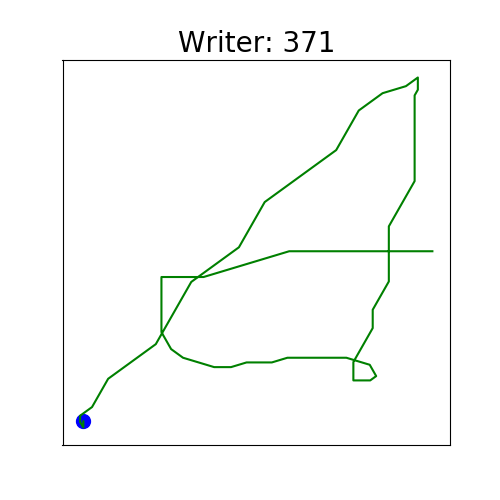
\includegraphics[scale=0.50]{images/framework/A_371.png}
      \end{subfigure}
      ~
      \begin{subfigure}{0.45\textwidth}
          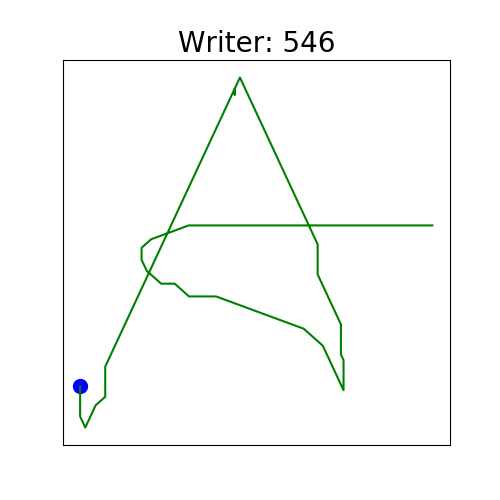
\includegraphics[scale=0.50]{images/framework/A_546.png}
      \end{subfigure}

      \caption{Examples for writing of letter A from the selected clusters. Starting point is marked with the blue mark. Each row is from one cluster. The first row show people who start drawing the letter from the top, going down, and then continue the drawing of the letter. The second row show people who start drawing from down directly.}
      \label{fig:examples_a}
  \end{figure}

  \begin{figure}[htbp!]
  \centering
  \fbox{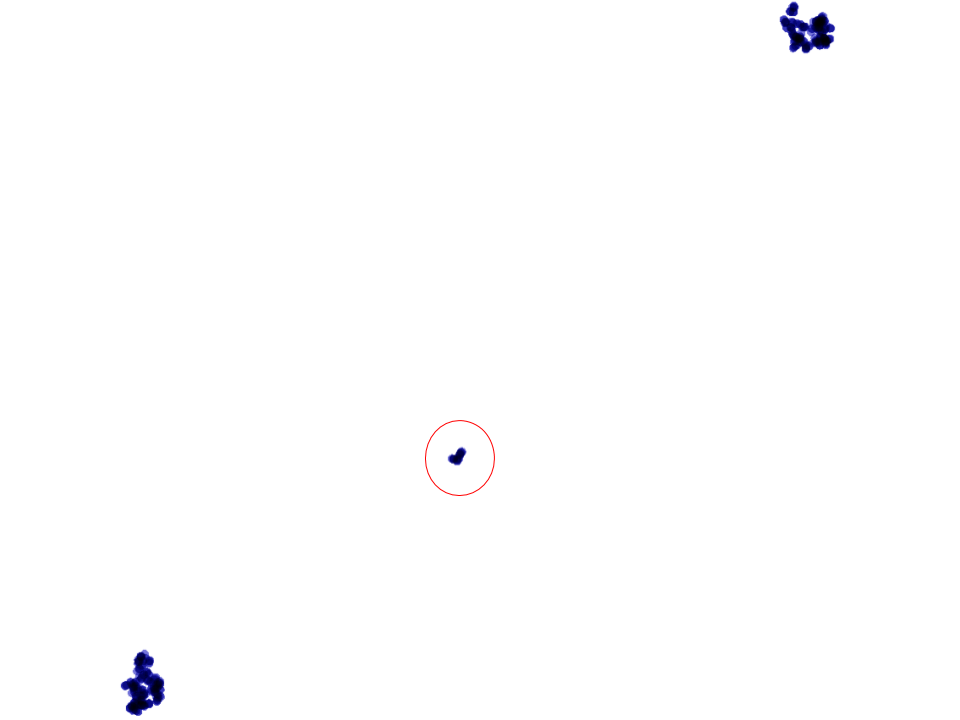
\includegraphics[scale=0.40]{images/framework/s_bottleneck.png}}
  \caption{Projection for latent space for letter S using t-SNE. We manage to interpret the indicated cluster as the Edwardian style in drawing. The other two clusters (not indicated) did not show clear difference in the style, but this is an expected behavior from using the t-SNE algorithm, since it does not try to cluster styles as an objective.}
  \label{fig:s_bottleneck}
  \end{figure}


  \begin{figure}[!htbp]
      \centering
      \begin{subfigure}{0.45\textwidth}
          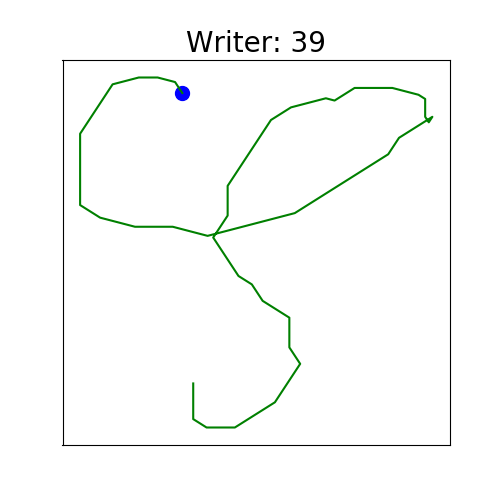
\includegraphics[scale=0.50]{images/framework/S_39.png}
      \end{subfigure}
      ~
      \begin{subfigure}{0.45\textwidth}
          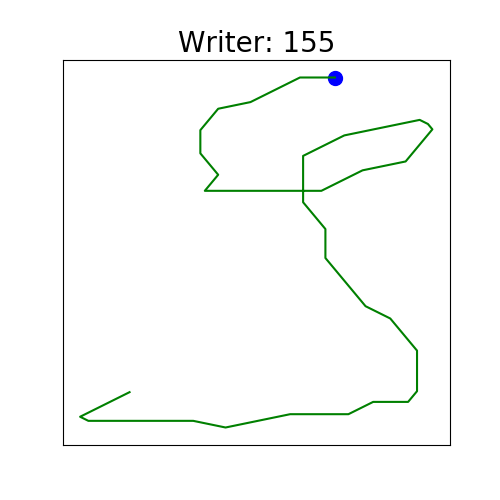
\includegraphics[scale=0.50]{images/framework/S_155.png}
      \end{subfigure}
      ~
      \begin{subfigure}{0.45\textwidth}
          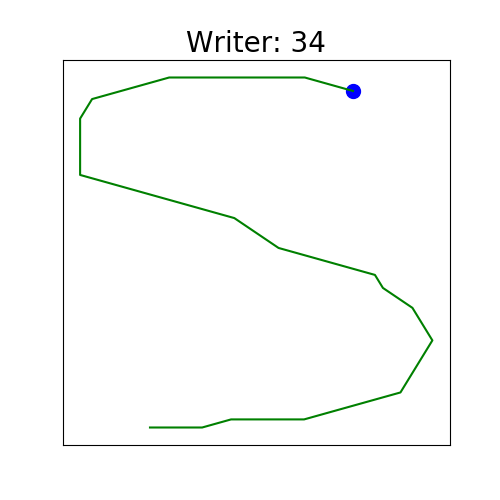
\includegraphics[scale=0.50]{images/framework/S_34.png}
      \end{subfigure}
      ~
      \begin{subfigure}{0.45\textwidth}
          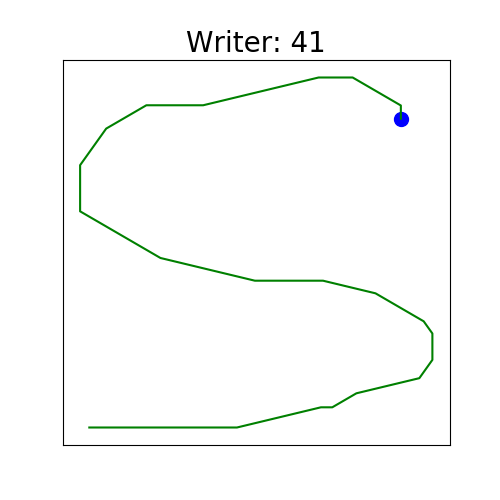
\includegraphics[scale=0.50]{images/framework/S_41.png}
      \end{subfigure}

      \caption{Examples for writing of letter S from the selected cluster (first row) versus the other two clusters (second row). Starting point is marked with the blue mark. The drawings from the selected cluster is always Edwardian style.}
      \label{fig:examples_s}
  \end{figure}

  \begin{sidewaysfigure}[!htbp]
  \centering
      \begin{subfigure}[b]{0.17\textwidth}
          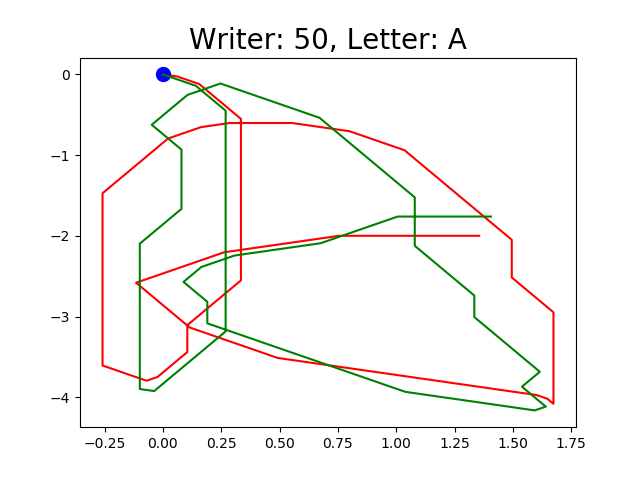
\includegraphics[width=\textwidth]{images/framework/comparison_figures/A_50.png}
      \end{subfigure}
      ~ %add desired spacing between images, e. g. ~, \quad, \qquad, \hfill etc.
        %(or a blank line to force the subfigure onto a new line)
      \begin{subfigure}[b]{0.17\textwidth}
          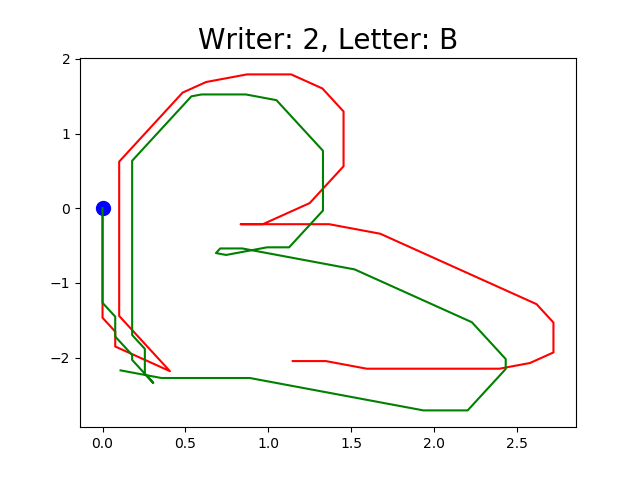
\includegraphics[width=\textwidth]{images/framework/comparison_figures/B_2.png}
      \end{subfigure}
      ~
      \begin{subfigure}[b]{0.17\textwidth}
          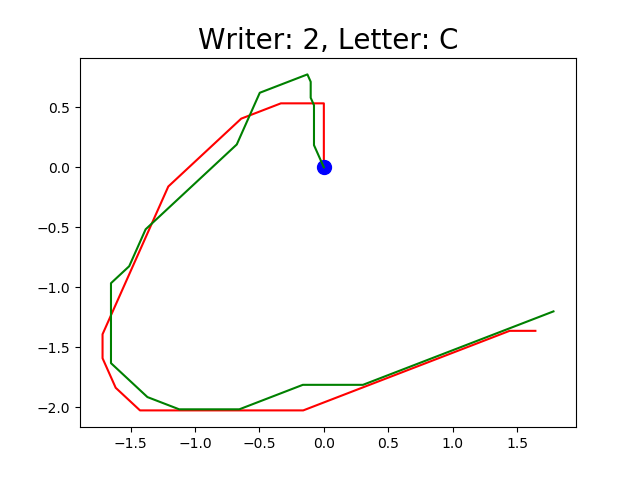
\includegraphics[width=\textwidth]{images/framework/comparison_figures/C_2.png}
      \end{subfigure}
      ~
      \begin{subfigure}[b]{0.17\textwidth}
          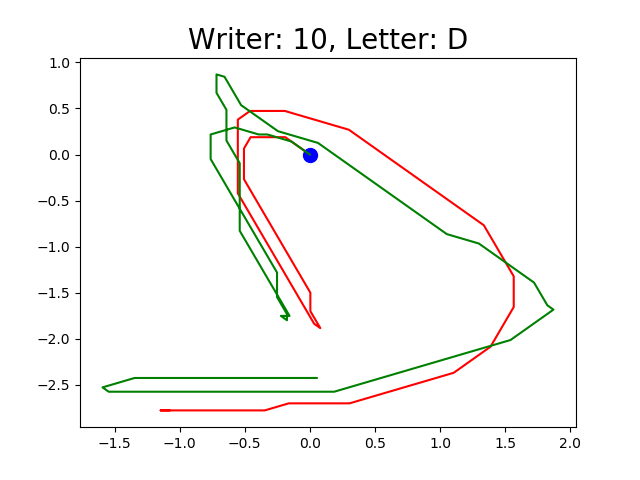
\includegraphics[width=\textwidth]{images/framework/comparison_figures/D_10.png}
      \end{subfigure}
      ~
      \begin{subfigure}[b]{0.17\textwidth}
          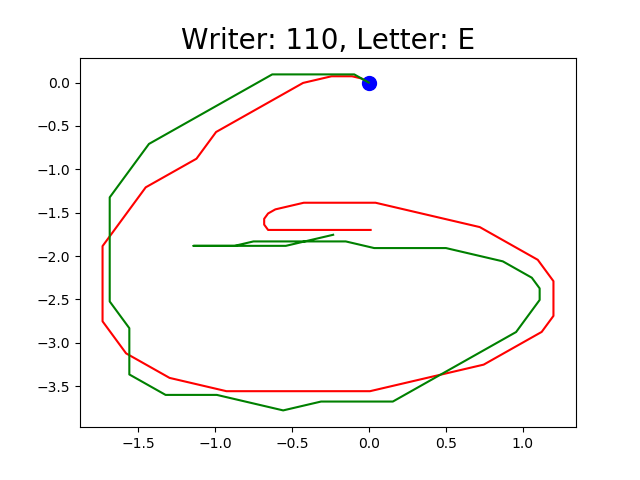
\includegraphics[width=\textwidth]{images/framework/comparison_figures/E_110.png}
      \end{subfigure}
      ~
      \begin{subfigure}[b]{0.17\textwidth}
          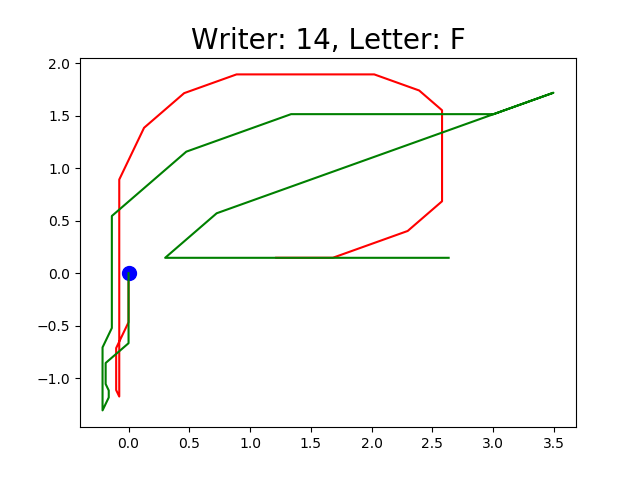
\includegraphics[width=\textwidth]{images/framework/comparison_figures/F_14.png}
      \end{subfigure}
      ~
      \begin{subfigure}[b]{0.17\textwidth}
          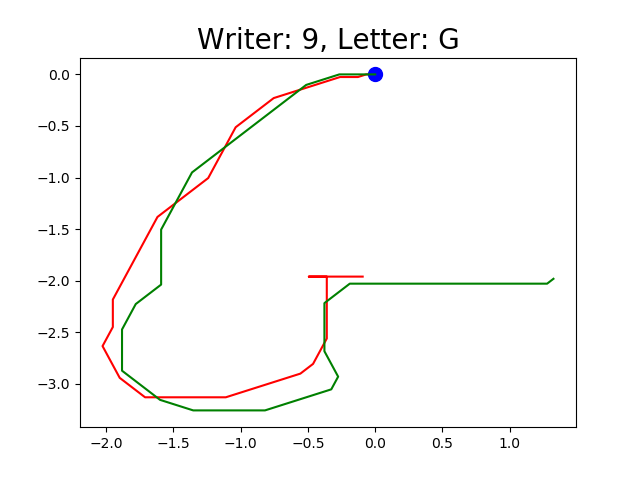
\includegraphics[width=\textwidth]{images/framework/comparison_figures/G_9.png}
      \end{subfigure}
      ~
      \begin{subfigure}[b]{0.17\textwidth}
          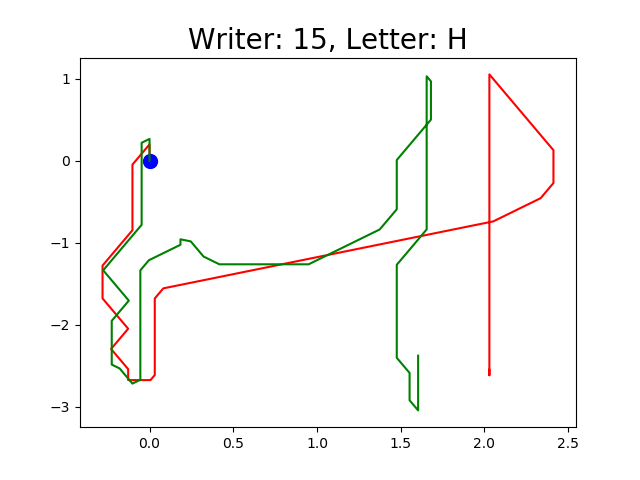
\includegraphics[width=\textwidth]{images/framework/comparison_figures/H_15.png}
      \end{subfigure}
      ~
      \begin{subfigure}[b]{0.17\textwidth}
          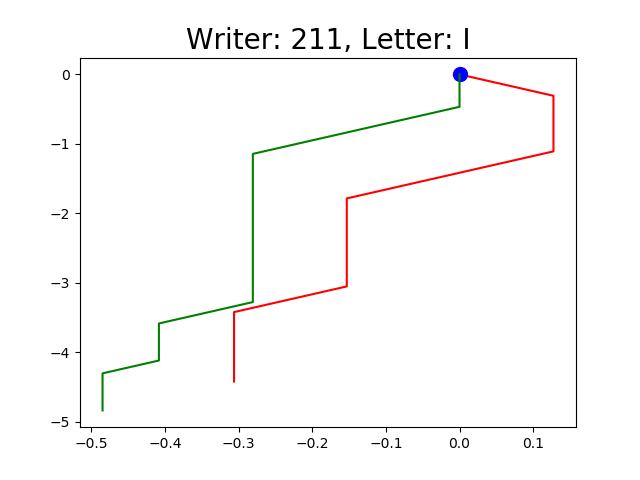
\includegraphics[width=\textwidth]{images/framework/comparison_figures/I_211.png}
      \end{subfigure}
      ~
      \begin{subfigure}[b]{0.17\textwidth}
          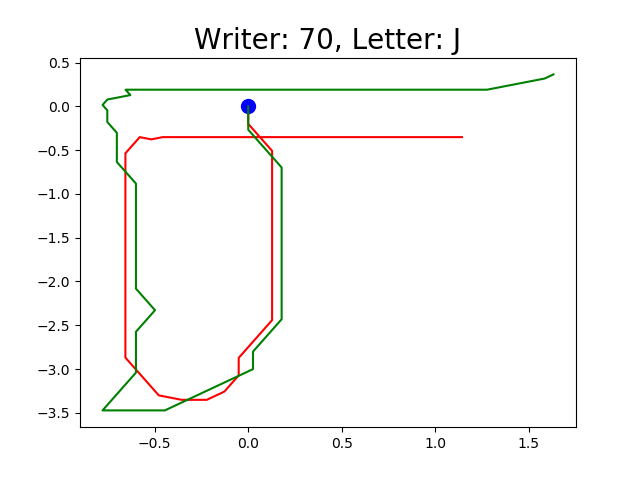
\includegraphics[width=\textwidth]{images/framework/comparison_figures/J_70.png}
      \end{subfigure}
      ~
      \begin{subfigure}[b]{0.17\textwidth}
          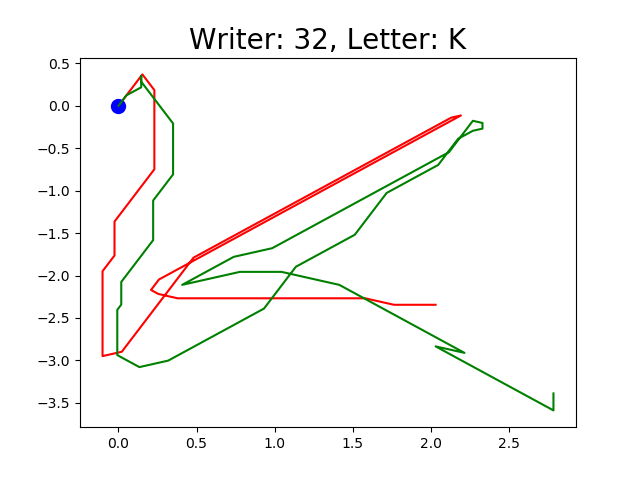
\includegraphics[width=\textwidth]{images/framework/comparison_figures/K_32.png}
      \end{subfigure}
      ~
      \begin{subfigure}[b]{0.17\textwidth}
          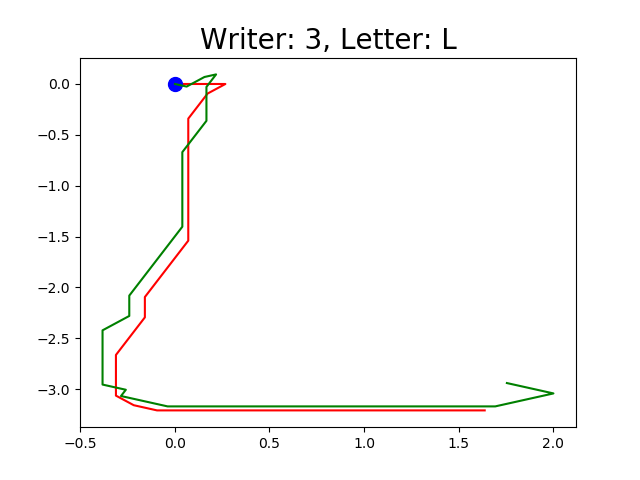
\includegraphics[width=\textwidth]{images/framework/comparison_figures/L_3.png}
      \end{subfigure}
      ~
      \begin{subfigure}[b]{0.17\textwidth}
          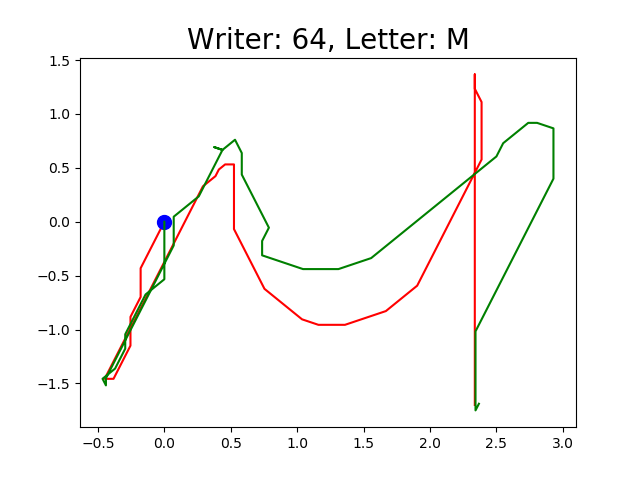
\includegraphics[width=\textwidth]{images/framework/comparison_figures/M_64.png}
      \end{subfigure}
      ~
      \begin{subfigure}[b]{0.17\textwidth}
          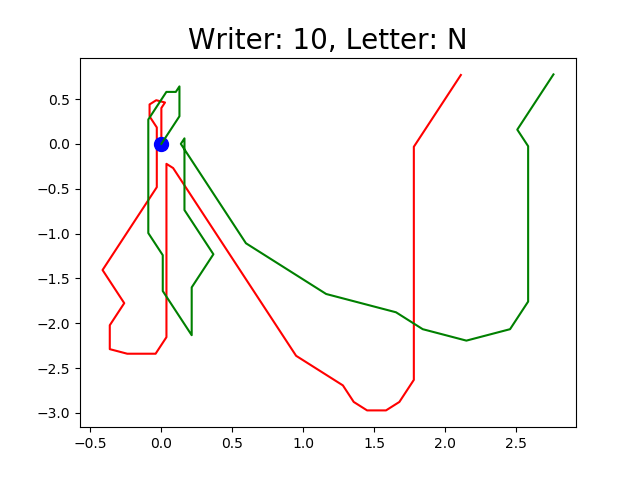
\includegraphics[width=\textwidth]{images/framework/comparison_figures/N_10.png}
      \end{subfigure}
      ~
      \begin{subfigure}[b]{0.17\textwidth}
          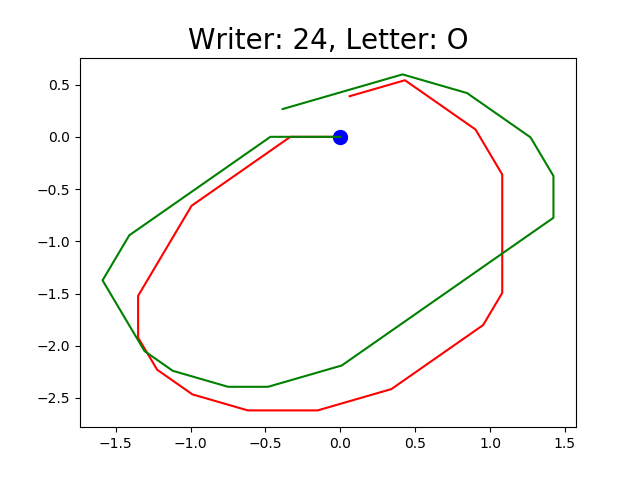
\includegraphics[width=\textwidth]{images/framework/comparison_figures/O_24.png}
      \end{subfigure}
      ~
      \begin{subfigure}[b]{0.17\textwidth}
          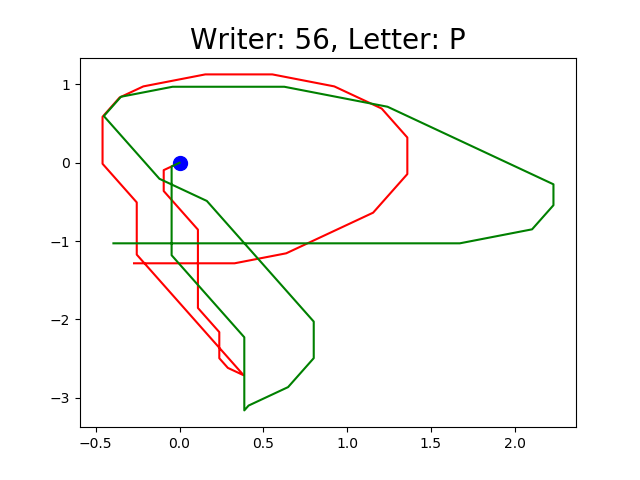
\includegraphics[width=\textwidth]{images/framework/comparison_figures/P_56.png}
      \end{subfigure}
      ~
      \begin{subfigure}[b]{0.17\textwidth}
          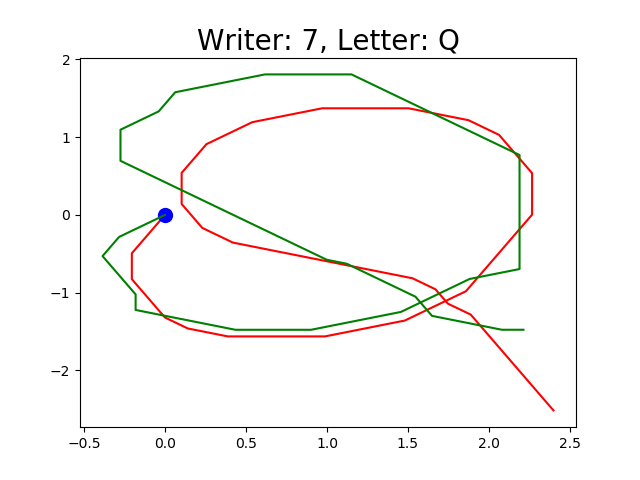
\includegraphics[width=\textwidth]{images/framework/comparison_figures/Q_7.png}
      \end{subfigure}
      ~
      \begin{subfigure}[b]{0.17\textwidth}
          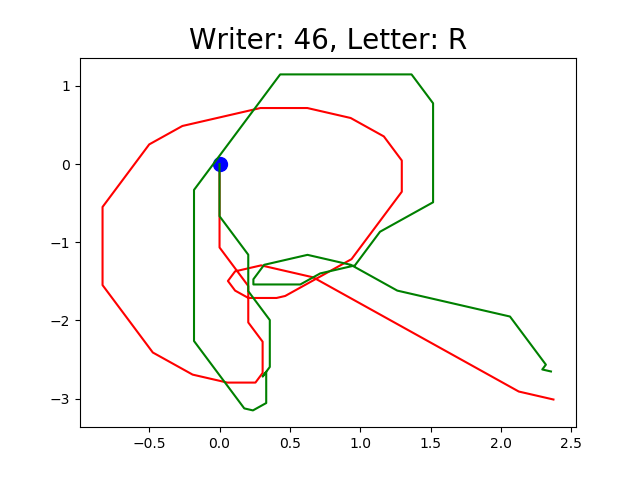
\includegraphics[width=\textwidth]{images/framework/comparison_figures/R_46.png}
      \end{subfigure}
      ~
      \begin{subfigure}[b]{0.17\textwidth}
          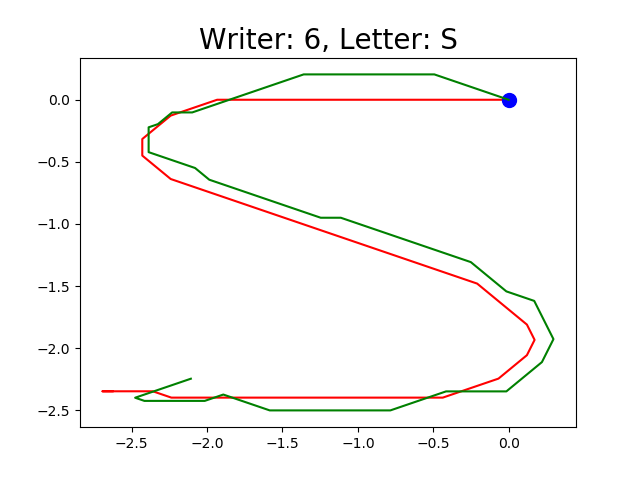
\includegraphics[width=\textwidth]{images/framework/comparison_figures/S_6.png}
      \end{subfigure}
      ~
      \begin{subfigure}[b]{0.17\textwidth}
          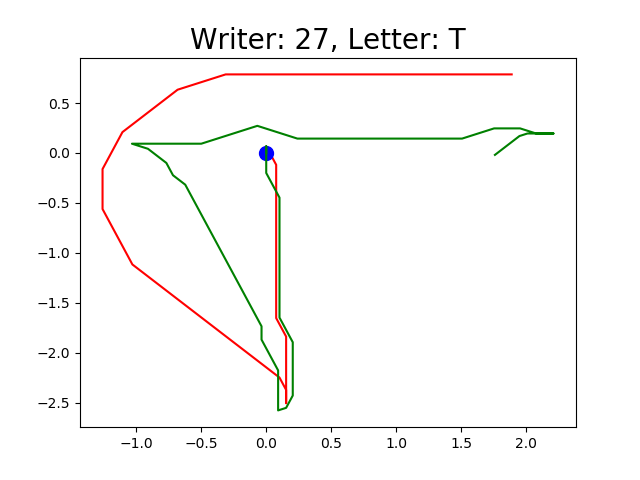
\includegraphics[width=\textwidth]{images/framework/comparison_figures/T_27.png}
      \end{subfigure}
      ~
      \begin{subfigure}[b]{0.17\textwidth}
          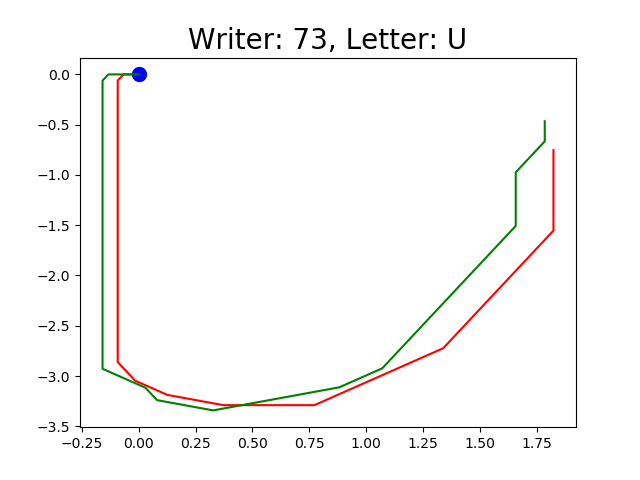
\includegraphics[width=\textwidth]{images/framework/comparison_figures/U_73.png}
      \end{subfigure}
      ~
      \begin{subfigure}[b]{0.17\textwidth}
          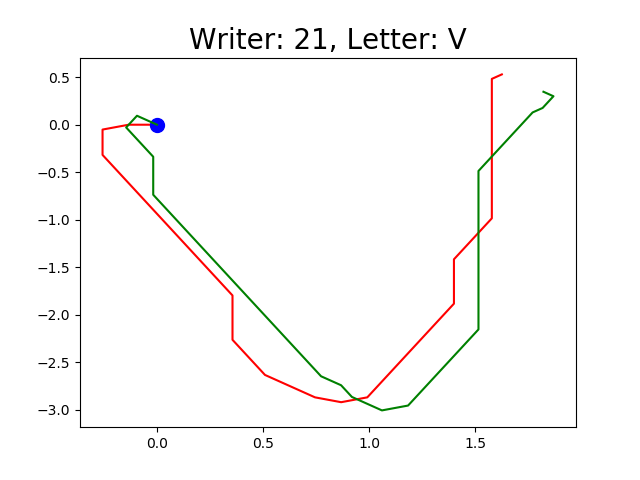
\includegraphics[width=\textwidth]{images/framework/comparison_figures/V_21.png}
      \end{subfigure}
      ~
      \begin{subfigure}[b]{0.17\textwidth}
          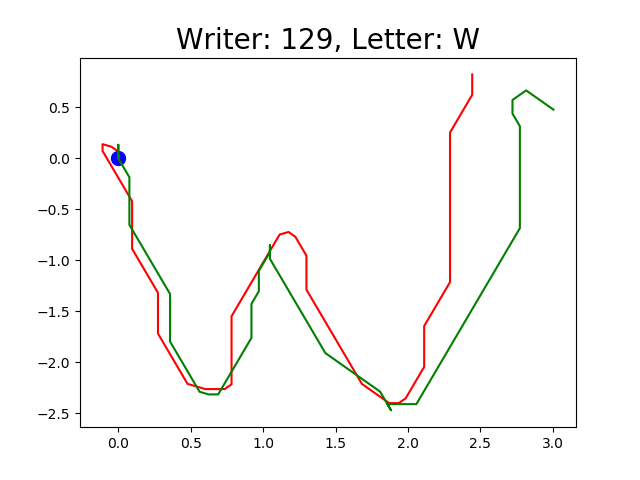
\includegraphics[width=\textwidth]{images/framework/comparison_figures/W_129.png}
      \end{subfigure}
      ~
      \begin{subfigure}[b]{0.17\textwidth}
          \includegraphics[width=\textwidth]{images/framework/comparison_figures/X_85.png}
      \end{subfigure}
      ~
      \begin{subfigure}[b]{0.17\textwidth}
          \includegraphics[width=\textwidth]{images/framework/comparison_figures/Y_24.png}
      \end{subfigure}
      ~
      \begin{subfigure}[b]{0.17\textwidth}
          \includegraphics[width=\textwidth]{images/framework/comparison_figures/Z_21.png}
      \end{subfigure}

      %%%%%%%%%%%%%%%%%%%%%%%%5
      %%%%%%%%%%%%%%%%%%%%%%%%%%%
      \caption{Examples of generated letters. The blue mark is the starting point. The traces in green is the ground truth, and the red is the generated ones by our model.}
      \label{fig:letters_examples}
  \end{sidewaysfigure}

  \begin{sidewaysfigure}[!htbp]
  \centering
      \begin{subfigure}[b]{0.17\textwidth}
          \includegraphics[width=\textwidth]{images/framework/comparison_figures/A_38.png}
      \end{subfigure}
      ~
      \begin{subfigure}[b]{0.17\textwidth}
          \includegraphics[width=\textwidth]{images/framework/comparison_figures/B_63.png}
      \end{subfigure}
      ~
      \begin{subfigure}[b]{0.17\textwidth}
          \includegraphics[width=\textwidth]{images/framework/comparison_figures/C_19.png}
      \end{subfigure}
      ~
      \begin{subfigure}[b]{0.17\textwidth}
          \includegraphics[width=\textwidth]{images/framework/comparison_figures/D_109.png}
      \end{subfigure}
      ~
      \begin{subfigure}[b]{0.17\textwidth}
          \includegraphics[width=\textwidth]{images/framework/comparison_figures/E_44.png}
      \end{subfigure}
      ~
      \begin{subfigure}[b]{0.17\textwidth}
          \includegraphics[width=\textwidth]{images/framework/comparison_figures/F_111.png}
      \end{subfigure}
      ~
      \begin{subfigure}[b]{0.17\textwidth}
          \includegraphics[width=\textwidth]{images/framework/comparison_figures/G_35.png}
      \end{subfigure}
      ~
      \begin{subfigure}[b]{0.17\textwidth}
          \includegraphics[width=\textwidth]{images/framework/comparison_figures/H_196.png}
      \end{subfigure}
      ~
      \begin{subfigure}[b]{0.17\textwidth}
          \includegraphics[width=\textwidth]{images/framework/comparison_figures/I_384.png}
      \end{subfigure}
      ~
      \begin{subfigure}[b]{0.17\textwidth}
          \includegraphics[width=\textwidth]{images/framework/comparison_figures/J_279.png}
      \end{subfigure}
      ~
      \begin{subfigure}[b]{0.17\textwidth}
          \includegraphics[width=\textwidth]{images/framework/comparison_figures/K_301.png}
      \end{subfigure}
      ~
      \begin{subfigure}[b]{0.17\textwidth}
          \includegraphics[width=\textwidth]{images/framework/comparison_figures/L_24.png}
      \end{subfigure}
      ~
      \begin{subfigure}[b]{0.17\textwidth}
          \includegraphics[width=\textwidth]{images/framework/comparison_figures/M_193.png}
      \end{subfigure}
      ~
      \begin{subfigure}[b]{0.17\textwidth}
          \includegraphics[width=\textwidth]{images/framework/comparison_figures/N_21.png}
      \end{subfigure}
      ~
      \begin{subfigure}[b]{0.17\textwidth}
          \includegraphics[width=\textwidth]{images/framework/comparison_figures/O_38.png}
      \end{subfigure}
      ~
      \begin{subfigure}[b]{0.17\textwidth}
          \includegraphics[width=\textwidth]{images/framework/comparison_figures/P_65.png}
      \end{subfigure}
      ~
      \begin{subfigure}[b]{0.17\textwidth}
          \includegraphics[width=\textwidth]{images/framework/comparison_figures/Q_140.png}
      \end{subfigure}
      ~
      \begin{subfigure}[b]{0.17\textwidth}
          \includegraphics[width=\textwidth]{images/framework/comparison_figures/R_91.png}
      \end{subfigure}
      ~
      \begin{subfigure}[b]{0.17\textwidth}
          \includegraphics[width=\textwidth]{images/framework/comparison_figures/S_125.png}
      \end{subfigure}
      ~
      \begin{subfigure}[b]{0.17\textwidth}
          \includegraphics[width=\textwidth]{images/framework/comparison_figures/T_84.png}
      \end{subfigure}
      ~
      \begin{subfigure}[b]{0.17\textwidth}
          \includegraphics[width=\textwidth]{images/framework/comparison_figures/U_83.png}
      \end{subfigure}
      ~
      \begin{subfigure}[b]{0.17\textwidth}
          \includegraphics[width=\textwidth]{images/framework/comparison_figures/V_32.png}
      \end{subfigure}
      ~
      \begin{subfigure}[b]{0.17\textwidth}
          \includegraphics[width=\textwidth]{images/framework/comparison_figures/W_191.png}
      \end{subfigure}
      ~
      \begin{subfigure}[b]{0.17\textwidth}
          \includegraphics[width=\textwidth]{images/framework/comparison_figures/X_187.png}
      \end{subfigure}
      ~
      \begin{subfigure}[b]{0.17\textwidth}
          \includegraphics[width=\textwidth]{images/framework/comparison_figures/Y_61.png}
      \end{subfigure}
      ~
      \begin{subfigure}[b]{0.17\textwidth}
          \includegraphics[width=\textwidth]{images/framework/comparison_figures/Z_383.png}
      \end{subfigure}
      %%%%%%%%%%%%%%%%%%%%%%%%5
      %%%%%%%%%%%%%%%%%%%%%%%%%%%
      \caption{Examples of generated letters. The blue mark is the starting point. The traces in green is the ground truth, and the red is the generated ones by our model.}
      \label{fig:letters_examples_2}
  \end{sidewaysfigure}

  \section{Summary}

    \par In this chapter, we discussed the way we chose in order to study styles, by using the auto-encoder framework. We hypothesized that we can study styles implicitly by looking at how they contribute to the reconstruction/generation of the letters. We looked at the state-of-the-art concerning auto-encoders, the sequence-to-sequence case, and why we may choose to condition an auto-encoder.

    \par I then presented our work, addressing the following points:
    \begin{itemize}
      \item What possible framework to study styles? And how to validate it? We test the auto-encoder framework relative the benchmarks we proposed in the previous chapter, in order to determine if it is actually a valid framework to study styles. We find that an auto-encoder outperforms the benchmarks in all evaluation metrics, suggesting that this is a good approach.
      \item What kind of styles we can extract from this framework? And how do we extract them? Given the good performance results of the auto-encoder, we wanted to have further confirmation that our model is actual learning relevant style information from one side, and if we can learn something new about styles. We explored the model bottleneck for different letters, showing a strong evidence that the model is quite useful in the study of styles.
      \item Can we transfer the styles over different writers? We hypothesis that there is a limited number of styles in general -- if we have enough writers in our training data, we will generalize well to new writers --. We test this hypothesis by hiding a number of writers from the training data, and compare a model trained on the other writers (transfer model) versus a model trained only on those writers (baseline model). We see clearly the transfer model outperforms the baseline, thus giving good evidence for our hypothesis.
    \end{itemize}

    We thus are ready for the next chapter, where we dive more into the world of transfer learning...
